% Бүлэг 2

\chapter{А.Эрдэнэбаатарын зөвлөмж} % Зарим нэг зөвлөмж

\label{Chapter2} % Энэ бүлэг рүү ишлэл хийх бол \ref{Chapter2} командыг ашигла 
\pagecolor{white}
%-------------------------------------------------------------------------------
%	SECTION 1
%-------------------------------------------------------------------------------

\section{Вектор зургийн тухай}

Зургийг растер, вектор гэж хоёр хувааж болно. Растер зургийг цэгээр бүтээдэг бөгөөд зургийн файл нь JPG, GIG, PNG г.м. өргөтгөсөн нэртэй байдаг. Түүнийг Adobe Photoshop мэтийн програмаар зурах, эсвэл зургийн аппарат зэрэг бусад эх үүсвэрээс авч болно. Бага нягтралтай растер зургийн хэмжээг ихэсгэхэд зургийн чанар алдагддаг. Чанарыг нь сайжруулъя гэвэл их нягтралтай байх хэрэгтэй. Ийм файл маш том болдог. Өмнөх бүлэг буюу Sunil Patel --н зөвлөмжөөс тезист ийм зургийн файлыг хэрхэн оруулахыг харсан.

Харин вектор зургийг цэгээр биш, математик томьёогоор илэрхийлсэн векторуудын нэгдэл байдлаар зурдаг. Ийм зураг маш бага зай эзэлдэг ба хэмжээг ихэсгэж/багасгахад чанар нь өөрчлөгддөггүй. Иймд түүнийг шинжлэх ухааны бүтээлд өргөн ашигладаг.

\LaTeX{} --д вектор зураг бүтээх олон тооны багц байдаг. Анх зурах техникийг эзэмших хэцүү мэт боловч сураад эхэлбэл растер зургийг тоохгүй болно.   

%-----------------------------------
%	SUBSECTION 1
%-----------------------------------
\subsection{TikZ багц}

\LaTeX{} --д зураг зурах олон янзын боломж байдаг. Энэ бүлэгт \code{\href{http://www.texample.net/tikz/examples/}{TikZ}} пакет ашиглаж зураг зурах зарим нэгэн жишээг үзнэ. 

Эхний жишээ бол төлөвийн автомат бөгөөд хэрхэн зурсныг \file{Chapter2.tex} файлаас харна уу. 
\begin{figure}[h]
\centering
\label{fig:automat}

\begin{tikzpicture}[->,>=stealth',shorten >=1pt,auto,node distance=2.8cm,
semithick]
\tikzstyle{every state}=[fill=red,draw=none,text=white]

\node[initial,state] (A)                    {$q_a$};
\node[state]         (B) [above right of=A] {$q_b$};
\node[state]         (D) [below right of=A] {$q_d$};
\node[state]         (C) [below right of=B] {$q_c$};
\node[state]         (E) [below of=D]       {$q_e$};

\path (A) edge              node {0,1,L} (B)
edge              node {1,1,R} (C)
(B) edge [loop above] node {1,1,L} (B)
edge              node {0,1,L} (C)
(C) edge              node {0,1,L} (D)
edge [bend left]  node {1,0,R} (E)
(D) edge [loop below] node {1,1,R} (D)
edge              node {0,1,R} (A)
(E) edge [bend left]  node {1,0,R} (A);
\end{tikzpicture}
\caption[Автомат]{Төлөвийн автомат.}
\end{figure}

Дараачийн жишээ бол энгийн блок схем.

\tikzstyle{decision} = [diamond, draw, fill=blue!20, 
    text width=7em, text badly centered, node distance=3cm, inner sep=0pt]
\tikzstyle{block} = [rectangle, draw, fill=blue!20, 
    text width=7em, text centered, rounded corners, minimum height=3em]
\tikzstyle{line} = [draw, -latex']
\tikzstyle{cloud} = [draw, ellipse, fill=red!20, node distance=4cm,
    minimum height=2em]
    
\begin{center}

\begin{tikzpicture}[node distance = 2cm, auto]
    % Place nodes
    \node [block] (init) {Загварыг идэвхижүүлэх};
    \node [cloud, left of=init] (expert) {Эксперт};
    \node [cloud, right of=init] (system) {Систем};
    \node [block, below of=init] (identify) {Шинэ загвар гаргах};
    \node [block, below of=identify] (evaluate) {Шинэ загварыг үнэлэх};
    \node [block, left of=evaluate, node distance=4cm] (update) {Загварыг шинэчлэх};
    \node [decision, below of=evaluate] (decide) {Загвар сайжирсан уу?};
    \node [block, below of=decide, node distance=3cm] (stop) {Төгсгөл};
    % Draw edges
    \path [line] (init) -- (identify);
    \path [line] (identify) -- (evaluate);
    \path [line] (evaluate) -- (decide);
    \path [line] (decide) -| node [near start] {тийм} (update);
    \path [line] (update) |- (identify);
    \path [line] (decide) -- node {үгүй}(stop);
    \path [line,dashed] (expert) -- (init);
    \path [line,dashed] (system) -- (init);
    \path [line,dashed] (system) |- (evaluate);
\end{tikzpicture}

\end{center}

%-----------------------------------
%	SECTION 2
%-----------------------------------

\section{Эх код хэвлэх}

\LaTeX{} -д програмын эх кодыг гоёор хэвлэх боломж бий. Үүнийг \code{listings} багцын тусламжтай хийж болно. Эх код програмчлалын ямар хэл дээр бичигдсэн болон бусад тохиргоог \file{main.tex} файлын эхэн хавьд байгаа \code{lstset} командаар тодорхойлно. Энэ багц \code{utf8} кодчиллыг дэмжихгүй тул эх код дотор орсон монгол текстийг гаргаж чадахгүй болохыг анхаарна уу.
  
\begin{lstlisting}[label=some-code,caption=Уламжлалт монгол тоглоом \enquote{Чулуу таалцах}]
/**
Mongolian traditional game "STONE GUESSING"
Players: Man, Computer1 and Computer2
**/
#include <stdio.h>
#include <stdlib.h>
#include <sys/time.h>

int main()
{
   int com1, com2, hum; // Players stones
   int nc1,nc2,nh; // Players fist stones
   int sum_c1,sum_c2,sum_h,sum; // Players guessing
   char ch;

   srand(time(NULL));

   Start:
   com1=com2=hum=10; // Initial number of stones

   while (1) { // Stone guessing
      if (hum == 0) { // "Man" in the game?
         nh=sum_h=0;
      }
      else {
         printf("\nPlease enter your stone number and sum of stones(Status %3d/%3d/%3d): ", com1,com2,hum);
         while (1) { // "Man" fist stones and guessing 
            scanf("%d%d", &nh, &sum_h);
            if ((nh >= 0 && nh <= hum) && (sum_h >= 0 && sum_h <= 30))
               break;
            else {
               printf("You enter wrong number(s). Try again:");
               continue;
            }
         }
      }

      if (com1 > 0) { // "Computer1" in the game?
         nc1=rand()%(com1+1);
         sum_c1=rand()%31; // Needs to improve "31"
      }
      else {
         nc1=sum_c1=0;
      }

      if (com2 > 0) { // "Computer2" in the game?
         nc2=rand()%(com2+1);
         sum_c2=rand()%31; // Needs to improve "31"
      }
      else {
         nc2=sum_c2=0;
      }

      sum=nc1+nc2+nh; // Sum of stones
      printf("         Com1  Com2  Hum   Sum\n");
      printf("Finger%6d%6d%6d%6d\n", nc1,nc2,nh,sum);
      printf("Sum   %6d%6d%6d\n", sum_c1,sum_c2,sum_h);

      if (sum == 0)
         continue;

      if (sum_c1 == sum && sum_h != sum && sum_c2 != sum) { // "Computer1" guessed
         printf("Winner%*s",6,"Win" );
         com1+=nh+nc2; hum-=nh; com2-=nc2;
         if (com1 == 30) {
            printf(" (Grand)\n");
            break;
         }
      }

      if (sum_c2 == sum && sum_h != sum && sum_c1 != sum) { // "Computer2" guessed
         printf("Winner%*s",12,"Win" );
         com2+=nh+nc1; hum-=nh; com1-=nc1;
         if (com2 == 30) {
            printf(" (Grand)\n");
            break;
         }
      }

      if (sum_h == sum && sum_c1 != sum && sum_c2 != sum) { // "Man" guessed
         printf("Winner%*s",18,"Win" );
         hum+=nc1+nc2; com1-=nc1; com2-=nc2;
         if (hum == 30) {
            printf(" (Grand)\n");
            break;
         }
      }
      printf("\n");

   } // End of while

   printf("\nDo you want to play again(Y -Yes/Others -No): "); // Play again?
   scanf(" %c", &ch);
   if (ch == 'Y' || ch == 'y')
      goto Start;

   return 0;
}

\end{lstlisting}

%-----------------------------------
%	SECTION 3
%-----------------------------------

\section{Зэрэгцээ болон том зураг}

Заримдаа хэд хэдэн зургийг нэг гарчигтай эвлүүлж харуулах хэрэг гардаг. 
\begin{figure} [!h]
\centering
\begin{minipage}{.5\textwidth}
	\centering
	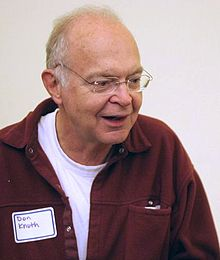
\includegraphics[width=0.8\linewidth]{Donald_Knuth.jpg}\\
	{Donald Knuth}
	\label{fig:knuth}
\end{minipage}%
\begin{minipage}{.5\textwidth}
	\centering
	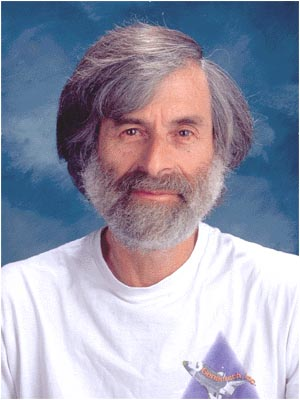
\includegraphics[width=0.75\linewidth]{Leslie_Lamport.jpg}\\
	{Leslie Lamport}
	\label{fig:lamport}
\end{minipage}
\caption{\LaTeX{} --ийн анхдагчид}
\end{figure}

\LaTeX{} --д том зургийг эргүүлээд тухайн (Зураг \ref{fig:MUST Enroll1}) болон бие даасан (Зураг \ref{fig:MUST Enroll2}) хуудас дээр хэвтээ байдлаар харуулж болно. 

\begin{figure}[!htbp]
	\centering
	\vspace{2mm}
	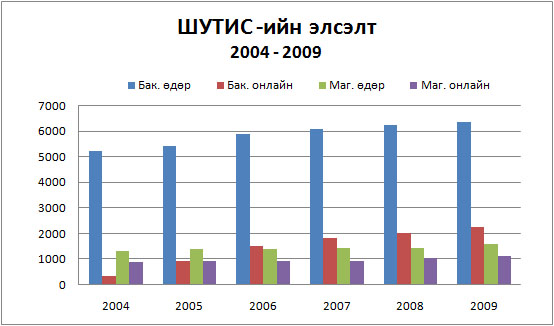
\includegraphics[scale=0.7,angle=90]{MUST_enrollment.jpg}
	\caption{ШУТИС-ийн элсэлт 2004 -- 2009 (эргүүлсэн)}
	\label{fig:MUST Enroll1}
\end{figure}

\begin{sidewaysfigure}[!htbp]
	\centering
	\vspace{2mm}
	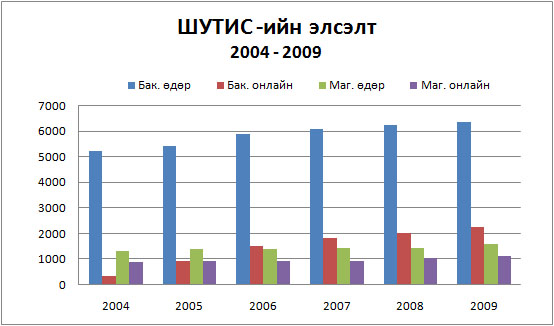
\includegraphics[scale=1.2]{MUST_enrollment.jpg}
	\caption{ШУТИС-ийн элсэлт 2004 -- 2009 (бүтэн хуудас)}
	\label{fig:MUST Enroll2}
\end{sidewaysfigure}

Эхний бүхнийг \file{Chapter2.tex} файлаас харна уу. 
